% Chapter 5: Forces and Motion
% For Stage 4 Science Textbook (Years 7-8, NSW Curriculum)
% Using Tufte-LaTeX document class

\documentclass[justified,notoc]{tufte-book}

% Essential packages
\usepackage[utf8]{inputenc}
\usepackage[T1]{fontenc}
\usepackage{graphicx}
\usepackage{amsmath,amssymb}
\usepackage[version=4]{mhchem} % For chemistry notation
\usepackage{booktabs} % For nice tables
\usepackage{microtype} % Better typography
\usepackage{tikz} % For diagrams
\usepackage{xcolor} % For colored text
\usepackage{soul} % For highlighting
\usepackage{tcolorbox} % For colored boxes
\usepackage{enumitem} % For better lists
\usepackage{wrapfig} % For wrapping text around figures
\usepackage{hyperref} % For links

% Custom colors
\definecolor{primary}{RGB}{0, 73, 144} % Deep blue
\definecolor{secondary}{RGB}{242, 142, 43} % Orange
\definecolor{highlight}{RGB}{255, 222, 89} % Yellow highlight
\definecolor{success}{RGB}{46, 139, 87} % Green
\definecolor{info}{RGB}{70, 130, 180} % Steel blue
\definecolor{note}{RGB}{220, 220, 220} % Light gray

% Custom commands for pedagogical elements
\newcommand{\keyword}[1]{\textbf{#1}\marginnote{\textbf{#1}: }}

\newcommand{\challengeicon}{★}
\newcommand{\challenge}[1]{\marginnote{\textbf{\challengeicon\ Challenge:} #1}}

\newcommand{\mathlink}[1]{\marginnote{\textbf{Math Link:} #1}}

\newcommand{\historylink}[1]{\marginnote{\textbf{History:} #1}}

\newenvironment{investigation}[1]{%
    \begin{tcolorbox}[colback=info!10,colframe=info,title=\textbf{Investigation: #1}]
}{%
    \end{tcolorbox}
}

\newenvironment{keyconcept}[1]{%
    \begin{tcolorbox}[colback=primary!5,colframe=primary,title=\textbf{Key Concept: #1}]
}{%
    \end{tcolorbox}
}

\newenvironment{tieredquestions}[1]{%
    \begin{tcolorbox}[colback=note!30,colframe=note!50,title=\textbf{Practice Questions - #1}]
}{%
    \end{tcolorbox}
}

\newenvironment{stopandthink}{%
    \begin{tcolorbox}[colback=highlight!30,colframe=highlight!50,title=\textbf{Stop and Think}]
}{%
    \end{tcolorbox}
}

\begin{document}

\chapter{Forces and Motion}

\begin{figure}
    \centering
    \fbox{\rule{0pt}{8cm}\rule{12cm}{0pt}}
    \caption{A collage showing different forces in action: a roller coaster (gravity and inertia), a sailing boat (wind force), and magnets repelling each other (magnetic force).}
\end{figure}

\section*{Chapter Overview}

\begin{quote}
    In this chapter, you will explore the fascinating world of forces and motion. You will learn how forces can make objects move, stop, or change direction, and discover the fundamental laws that govern motion in our universe. Through hands-on investigations, you will observe forces like gravity, friction, and magnetism, and understand how these forces impact our daily lives—from sports to transportation and beyond.
\end{quote}

\noindent This chapter aligns with the following NSW Syllabus outcomes:
\begin{itemize}
    \item SC4-10PW: Describes the action of unbalanced forces in everyday situations
    \item SC4-11PW: Discusses how scientific understanding and technological developments have contributed to finding solutions to problems involving energy transfers and transformations
    \item SC4-7WS: Processes and analyses data from a first-hand investigation and secondary sources to identify trends, patterns and relationships, and draw conclusions
\end{itemize}

\newthought{Before we begin}, let's check what you already know about forces and motion. Take a moment to answer these questions:

\begin{stopandthink}
\begin{enumerate}
    \item What happens when you push or pull an object?
    \item Why does a ball rolling on the ground eventually stop?
    \item What causes objects to fall to the ground?
    \item Name three examples of forces you encounter in everyday life.
\end{enumerate}
\end{stopandthink}

\section{What Are Forces?}

\newthought{Forces} are pushes or pulls that act on objects.
\marginnote{The word "force" comes from the Latin word "fortis," meaning strong.}
When you push a door open, kick a football, or lift your backpack, you are applying a force. Forces can make objects start moving, stop moving, change speed, or change direction.

\keyword{Force} is defined as a push or pull that can change the motion of an object. Forces are measured in units called \keyword{newtons} (N), named after the scientist Sir Isaac Newton.

\historylink{Sir Isaac Newton (1643-1727) was one of history's most influential scientists. His three laws of motion, published in 1687, formed the foundation of classical mechanics.}

\subsection{Types of Forces}

Forces can be categorized in different ways, but one useful classification is:

\begin{keyconcept}{Contact vs. Non-Contact Forces}
\begin{description}
    \item[Contact forces] require physical contact between objects. Examples include:
    \begin{itemize}
        \item Pushing or pulling (applied forces)
        \item Friction
        \item Air resistance
        \item Tension (in strings, ropes)
        \item Spring forces
    \end{itemize}

    \item[Non-contact forces] act between objects that are not touching. Examples include:
    \begin{itemize}
        \item Gravity
        \item Magnetism
        \item Electrostatic forces
    \end{itemize}
\end{description}
\end{keyconcept}

\begin{marginfigure}
    \centering
    \fbox{\rule{0pt}{4cm}\rule{6cm}{0pt}}
    \caption{Examples of contact forces (top) and non-contact forces (bottom).}
\end{marginfigure}

\subsection{Representing Forces}

Scientists use arrows called \keyword{force vectors} to represent forces in diagrams. The direction of the arrow shows the direction of the force, and the length of the arrow represents the strength or magnitude of the force.

\begin{figure}
    \centering
    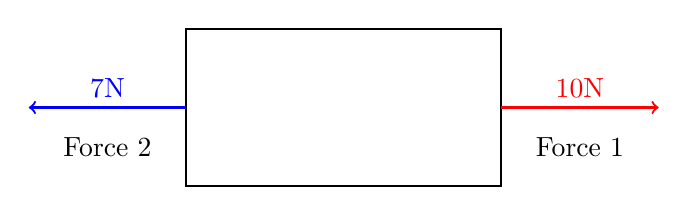
\begin{tikzpicture}
        % Draw a box
        \draw[thick] (0,0) rectangle (4,2);

        % Draw force arrows
        \draw[->,thick,red] (4,1) -- (6,1) node[midway,above] {10N};
        \draw[->,thick,blue] (0,1) -- (-2,1) node[midway,above] {7N};

        % Label the forces
        \node at (5,0.5) {Force 1};
        \node at (-1,0.5) {Force 2};
    \end{tikzpicture}
    \caption{Force vectors showing two forces acting on a box in opposite directions. The red arrow (Force 1) represents a 10N force pushing right, while the blue arrow (Force 2) represents a 7N force pushing left.}
\end{figure}

\challenge{Draw force vectors to represent the forces acting on a book sitting on a table. Include gravity pulling down and the table pushing up (called the normal force). What would happen if these forces weren't equal?}

\section{Balanced and Unbalanced Forces}

\newthought{When multiple forces} act on an object, they can either be balanced or unbalanced.

\subsection{Balanced Forces}

\keyword{Balanced forces} occur when all the forces acting on an object cancel each other out, resulting in a net force of zero. When forces are balanced:
\begin{itemize}
    \item If the object is stationary, it remains stationary.
    \item If the object is moving at a constant speed in a straight line, it continues moving at that same speed and direction.
\end{itemize}

\begin{marginfigure}
    \centering
    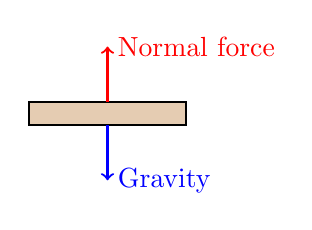
\begin{tikzpicture}
        % Draw a book
        \draw[thick,fill=brown!40] (0,0) rectangle (2,0.3);

        % Draw force arrows
        \draw[->,thick,red] (1,0.3) -- (1,1) node[right] {Normal force};
        \draw[->,thick,blue] (1,0) -- (1,-0.7) node[right] {Gravity};
    \end{tikzpicture}
    \caption{A book at rest on a table experiences balanced forces. The normal force pushing up equals the gravitational force pulling down.}
\end{marginfigure}

\begin{example}
A book sitting on a table is not moving. This is because the gravitational force pulling down on the book is exactly balanced by the normal force of the table pushing up.
\end{example}

\subsection{Unbalanced Forces}

\keyword{Unbalanced forces} occur when the forces acting on an object do not cancel out, resulting in a non-zero net force. When forces are unbalanced:
\begin{itemize}
    \item If the object is stationary, it starts moving in the direction of the net force.
    \item If the object is already moving, it changes its speed or direction or both.
\end{itemize}

\begin{marginfigure}
    \centering
    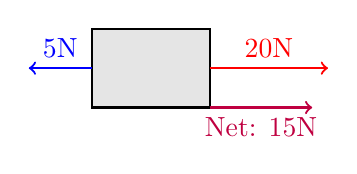
\begin{tikzpicture}
        % Draw a box
        \draw[thick,fill=gray!20] (0,0) rectangle (1.5,1);

        % Draw force arrows
        \draw[->,thick,red] (1.5,0.5) -- (3,0.5) node[midway,above] {20N};
        \draw[->,thick,blue] (0,0.5) -- (-0.8,0.5) node[midway,above] {5N};

        % Draw net force
        \draw[->,thick,purple] (1.5,0) -- (2.8,0) node[midway,below] {Net: 15N};
    \end{tikzpicture}
    \caption{A box with unbalanced forces. The net force is 15N to the right, causing the box to accelerate in that direction.}
\end{marginfigure}

\begin{example}
When you kick a ball, you apply an unbalanced force to it. This causes the ball to change from being stationary to moving in the direction of your kick.
\end{example}

\mathlink{To calculate the net force, add all forces acting in the same direction, then subtract the forces acting in the opposite direction.}

\begin{investigation}{Balanced vs. Unbalanced Forces}
\textbf{Materials:}
\begin{itemize}
    \item A toy car or wooden block
    \item String
    \item Small weights or coins
    \item Smooth surface (table or floor)
\end{itemize}

\textbf{Procedure:}
\begin{enumerate}
    \item Attach a string to the front of the car/block and another string to the back.
    \item Place the car/block on a smooth surface.
    \item Have one person pull on one string with a gentle, constant force.
    \item Have another person pull on the other string with an equal force in the opposite direction.
    \item Observe what happens to the car/block.
    \item Now have one person pull harder than the other. Observe what happens.
    \item Try different combinations of forces and record your observations.
\end{enumerate}

\textbf{Questions:}
\begin{enumerate}
    \item What happened when equal forces were applied in opposite directions?
    \item What happened when unequal forces were applied?
    \item How is this demonstration related to Newton's First Law of Motion?
    \item Can you think of three real-life examples where balanced forces keep objects stationary?
\end{enumerate}
\end{investigation}

\section{Newton's First Law of Motion}

\newthought{Isaac Newton formulated} three fundamental laws that describe how forces affect motion. The first of these laws is particularly relevant to our understanding of balanced and unbalanced forces.

\begin{keyconcept}{Newton's First Law of Motion}
An object at rest will stay at rest, and an object in motion will stay in motion with the same speed and in the same direction, unless acted upon by an unbalanced force.
\end{keyconcept}

Newton's First Law is sometimes called the \keyword{Law of Inertia}. \keyword{Inertia} is the resistance of an object to changes in its state of motion.
\marginnote{The more mass an object has, the greater its inertia. This is why it's harder to start or stop a heavy shopping cart than an empty one.}

\begin{figure}
    \centering
    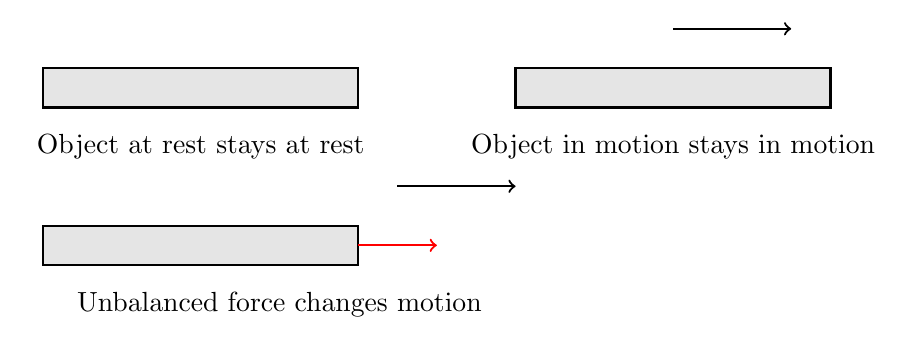
\begin{tikzpicture}
        % First scenario - object at rest
        \fill[gray!20] (-4,0) rectangle (0,0.5);
        \draw[thick] (-4,0) rectangle (0,0.5);
        \node at (-2,-0.5) {Object at rest stays at rest};

        % Second scenario - object in motion
        \fill[gray!20] (2,0) rectangle (6,0.5);
        \draw[thick] (2,0) rectangle (6,0.5);
        \draw[->,thick] (4,1) -- (5.5,1);
        \node at (4,-0.5) {Object in motion stays in motion};

        % Third scenario - unbalanced force
        \fill[gray!20] (-4,-2) rectangle (0,-1.5);
        \draw[thick] (-4,-2) rectangle (0,-1.5);
        \draw[->,thick,red] (0,-1.75) -- (1,-1.75);
        \draw[->,thick] (0.5,-1) -- (2,-1);
        \node at (-1,-2.5) {Unbalanced force changes motion};
    \end{tikzpicture}
    \caption{Illustrations of Newton's First Law: An object at rest stays at rest, an object in motion stays in motion, and an unbalanced force changes an object's motion.}
\end{figure}

\subsection{Real-Life Examples of Newton's First Law}

Newton's First Law explains many everyday phenomena:

\begin{itemize}
    \item \textbf{Seat belts in cars:} When a car stops suddenly, your body tends to keep moving forward (inertia) until restrained by the seat belt.

    \item \textbf{Setting a table:} When you quickly pull a tablecloth from under dishes, the dishes tend to stay in place due to inertia (if done correctly!).

    \item \textbf{Sports:} A football continues to move after being kicked until forces like friction and air resistance slow it down.
\end{itemize}

\challenge{Design a simple experiment to demonstrate Newton's First Law using everyday materials. Explain what materials you would use, what you would do, and what you would expect to observe.}

\section{Common Forces in Everyday Life}

\newthought{Several forces affect} our daily lives in countless ways. Let's explore some of the most common ones.

\subsection{Gravity}

\keyword{Gravity} is a non-contact force that attracts objects with mass toward each other. On Earth, gravity pulls objects toward the center of the planet.
\marginnote{The acceleration due to gravity on Earth is approximately 9.8 meters per second squared $(9.8 \text{ m/s}^2)$.}

The force of gravity (weight) on an object depends on its mass:

\begin{equation}
\text{Weight} = \text{mass} \times \text{gravity}
\end{equation}

Or, using symbols:

\begin{equation}
W = m \times g
\end{equation}

Where:
\begin{itemize}
    \item $W$ is weight in newtons (N)
    \item $m$ is mass in kilograms (kg)
    \item $g$ is the acceleration due to gravity $(9.8 \text{ m/s}^2)$
\end{itemize}

\mathlink{A 5 kg object on Earth weighs $5 \text{ kg} \times 9.8 \text{ m/s}^2 = 49 \text{ N}$. The same object on the Moon would weigh only about 8.3 N because the Moon's gravity is approximately 1/6 of Earth's.}

\historylink{The story of Newton discovering gravity when an apple fell from a tree is likely embellished, but Newton did use the concept of falling objects in developing his theory of universal gravitation.}

\subsection{Friction}

\keyword{Friction} is a contact force that opposes motion between two surfaces that are in contact with each other.
\marginnote{Without friction, we couldn't walk, drive cars, or hold objects!}

Types of friction include:
\begin{itemize}
    \item \textbf{Static friction:} Prevents objects from starting to move
    \item \textbf{Sliding friction:} Acts when objects slide against each other
    \item \textbf{Rolling friction:} Acts when objects roll against each other
    \item \textbf{Fluid friction:} Resistance in liquids and gases (e.g., air resistance)
\end{itemize}

Factors that affect friction include:
\begin{itemize}
    \item The types of surfaces in contact (rough vs. smooth)
    \item How hard the surfaces press together (normal force)
    \item Whether the object is rolling or sliding
\end{itemize}

\begin{investigation}{Investigating Friction}
\textbf{Materials:}
\begin{itemize}
    \item Wooden block or book
    \item Spring scale or force meter
    \item Various surfaces (carpet, tile, sandpaper, waxed paper)
    \item Weights to add to the block
\end{itemize}

\textbf{Procedure:}
\begin{enumerate}
    \item Place the block on one of the surfaces.
    \item Attach the spring scale/force meter to the block.
    \item Pull horizontally with a slow, steady force until the block just starts to move.
    \item Record the force required to start the block moving (static friction).
    \item Record the force required to keep the block moving at a constant speed (sliding friction).
    \item Repeat with different surfaces.
    \item Add weights to the block and repeat the measurements.
\end{enumerate}

\textbf{Questions:}
\begin{enumerate}
    \item Which surface had the most friction? Which had the least?
    \item How did adding weight affect the amount of friction?
    \item How is friction both helpful and harmful in everyday life?
    \item Design an experiment to test how you could reduce friction between two surfaces.
\end{enumerate}
\end{investigation}

\subsection{Magnetic Forces}

\keyword{Magnetic force} is a non-contact force exerted by magnets or moving electric charges.
\marginnote{Only certain materials respond to magnets. Iron, nickel, and cobalt are common magnetic materials.}

Key points about magnets:
\begin{itemize}
    \item Magnets have two poles: north and south
    \item Like poles repel each other; opposite poles attract
    \item Magnetic force acts through space (no physical contact needed)
    \item Magnetic force decreases with distance
\end{itemize}

\begin{marginfigure}
    \centering
    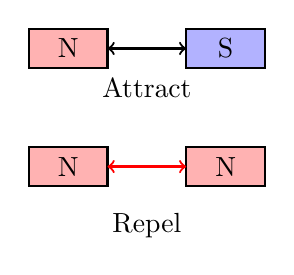
\begin{tikzpicture}
        % Draw two magnets attracting
        \draw[thick,fill=red!30] (0,0) rectangle (1,0.5);
        \draw[thick,fill=blue!30] (2,0) rectangle (3,0.5);
        \node at (0.5,0.25) {N};
        \node at (2.5,0.25) {S};
        \draw[<->,thick] (1,0.25) -- (2,0.25);
        \node at (1.5,-0.25) {Attract};

        % Draw two magnets repelling
        \draw[thick,fill=red!30] (0,-1.5) rectangle (1,-1);
        \draw[thick,fill=red!30] (2,-1.5) rectangle (3,-1);
        \node at (0.5,-1.25) {N};
        \node at (2.5,-1.25) {N};
        \draw[<->,thick,red] (1,-1.25) -- (2,-1.25);
        \node at (1.5,-2) {Repel};
    \end{tikzpicture}
    \caption{Magnetic attraction and repulsion: opposite poles attract, while like poles repel.}
\end{marginfigure}

\begin{investigation}{Exploring Magnetic Force}
\textbf{Materials:}
\begin{itemize}
    \item Two bar magnets
    \item Various small objects (paper clips, coins, rubber bands, aluminum foil, etc.)
    \item Ruler
    \item String
\end{itemize}

\textbf{Procedure (Part 1 - Attraction/Repulsion):}
\begin{enumerate}
    \item Place one magnet on the table.
    \item Slowly bring the north pole of the second magnet toward the north pole of the first magnet.
    \item Observe what happens and record the distance at which you feel the force.
    \item Repeat with north pole to south pole.
    \item Compare the forces of attraction and repulsion.
\end{enumerate}

\textbf{Procedure (Part 2 - Testing Materials):}
\begin{enumerate}
    \item Test each object by bringing a magnet close to it.
    \item Sort the objects into "magnetic" and "non-magnetic" groups.
    \item For magnetic objects, determine the maximum distance at which the magnet can attract them.
\end{enumerate}

\textbf{Questions:}
\begin{enumerate}
    \item What patterns did you notice about which materials are attracted to magnets?
    \item How does distance affect magnetic force?
    \item How are magnets used in everyday technology? List at least three examples.
\end{enumerate}
\end{investigation}

\section{Forces in Action}

\newthought{Forces shape} virtually every activity in our lives. Let's look at some contexts where understanding forces helps us explain everyday phenomena.

\subsection{Forces in Sports}

Sports provide excellent examples of forces in action:

\begin{itemize}
    \item \textbf{Swimming:} Swimmers push water backward to propel themselves forward (action-reaction forces).

    \item \textbf{Tennis:} When a racket hits a ball, it applies a force that changes the ball's direction and speed.

    \item \textbf{Skateboarding:} Skateboarders use a pushing force against the ground to move forward, while gravity pulls them down and friction helps them control their movement.
\end{itemize}

\begin{marginfigure}
    \centering
    \fbox{\rule{0pt}{4cm}\rule{6cm}{0pt}}
    \caption{Forces in action during a tennis serve. Multiple forces include the player's muscular force, gravity, and the racket's impact force on the ball.}
\end{marginfigure}

\subsection{Forces in Transportation}

Transportation systems rely on forces:

\begin{itemize}
    \item \textbf{Cars:} Engine provides forward force, friction between tires and road enables movement, brakes create opposing force to slow down.

    \item \textbf{Airplanes:} Four main forces: thrust (forward), drag (backward), lift (upward), and weight (downward).

    \item \textbf{Boats:} Buoyancy counters weight, propellers provide thrust, water resistance creates drag.
\end{itemize}

\challenge{Research how Newton's laws of motion apply to rocket launches. How do rockets use forces to escape Earth's gravity?}

\subsection{Forces and Safety}

Understanding forces is crucial for designing safety features:

\begin{itemize}
    \item \textbf{Seat belts and air bags:} Extend the time of impact during a collision, reducing the force on passengers.

    \item \textbf{Helmets:} Absorb impact forces to protect the head.

    \item \textbf{Crumple zones in cars:} Designed to collapse during a collision, absorbing energy and reducing forces transmitted to passengers.
\end{itemize}

\begin{keyconcept}{Force, Time, and Safety}
For a given change in momentum, extending the time of impact reduces the force experienced. This principle is the basis for many safety designs.

$\text{Force} = \frac{\text{Change in momentum}}{\text{Time}}$
\end{keyconcept}

\section{Chapter Review and Practice}

\newthought{Let's review} the key concepts we've covered in this chapter:

\begin{enumerate}
    \item Forces are pushes or pulls that can change the motion of objects
    \item Forces can be contact forces or non-contact forces
    \item Balanced forces result in no change in motion
    \item Unbalanced forces cause changes in motion (acceleration)
    \item Newton's First Law: objects remain at rest or in uniform motion unless acted upon by an unbalanced force
    \item Common forces include gravity, friction, and magnetism
    \item Forces play important roles in sports, transportation, and safety
\end{enumerate}

\begin{tieredquestions}{Level 1 - Basic Understanding}
\begin{enumerate}
    \item Define what a force is and give three examples.
    \item Distinguish between contact forces and non-contact forces.
    \item Explain what happens to an object when:
    \begin{enumerate}
        \item Forces acting on it are balanced
        \item Forces acting on it are unbalanced
    \end{enumerate}
    \item State Newton's First Law of Motion in your own words.
    \item Calculate the weight of a 10 kg object on Earth.
\end{enumerate}
\end{tieredquestions}

\begin{tieredquestions}{Level 2 - Application}
\begin{enumerate}
    \item A book is sliding across a table and gradually slows to a stop. Explain this observation in terms of forces and Newton's First Law.
    \item Two students are pulling on opposite ends of a rope. Student A pulls with 50N of force to the right. Student B pulls with 50N of force to the left. What is the net force on the rope? What will happen to the rope?
    \item Explain how friction can be both helpful and harmful using examples from everyday life.
    \item A roller coaster moves through a vertical loop. Identify all the forces acting on the roller coaster car at the top of the loop and explain why the passengers don't fall out.
    \item Design an experiment to measure the effect of surface area on friction.
\end{enumerate}
\end{tieredquestions}

\begin{tieredquestions}{Level 3 - Extension and Analysis}
\begin{enumerate}
    \item Research antigravity and evaluate whether it's scientifically possible based on our current understanding of physics.
    \item Compare the effects of friction on Earth with those on the Moon or in the International Space Station. How would everyday activities differ in these environments?
    \item Design a Rube Goldberg machine that demonstrates at least three different types of forces. Explain the forces involved at each stage.
    \item Analyze the forces involved in a sport of your choice. Create a diagram showing these forces and explain how understanding physics could help improve performance in this sport.
    \item Investigate how animals use forces in nature (e.g., how geckos climb walls, how birds fly). Choose one example and explain the physics involved.
\end{enumerate}
\end{tieredquestions}

\section{Glossary of Key Terms}

\begin{description}
    \item[Acceleration] The rate of change of velocity; occurs when an object speeds up, slows down, or changes direction.
    \item[Balanced forces] Forces that cancel each other out, resulting in no change in motion.
    \item[Contact force] A force that requires physical contact between objects.
    \item[Force] A push or pull that can change the motion of an object.
    \item[Friction] A force that opposes motion between surfaces that are in contact.
    \item[Gravity] A non-contact force that attracts objects with mass toward each other.
    \item[Inertia] The tendency of an object to resist changes in its state of motion.
    \item[Magnetic force] A non-contact force exerted by magnets or moving electric charges.
    \item[Newton (N)] The SI unit of force. One newton is the force needed to accelerate 1 kg of mass at 1 m/s².
    \item[Non-contact force] A force that acts between objects that are not touching.
    \item[Unbalanced forces] Forces that do not cancel out, resulting in a change in motion.
    \item[Weight] The force of gravity acting on an object; equal to mass times the acceleration due to gravity.
\end{description}

\section{Beyond the Basics: Exploring Further}

\newthought{Want to learn more?} Here are some suggestions for further exploration:

\begin{itemize}
    \item \textbf{Research Project:} Investigate how engineers use their understanding of forces to design roller coasters, bridges, or buildings.

    \item \textbf{Citizen Science:} Measure and compare friction coefficients for different household surfaces.

    \item \textbf{Digital Exploration:} Use physics simulation software (like PhET simulations) to experiment with forces and motion in virtual environments.

    \item \textbf{STEM Career Connection:} Interview an engineer, physicist, or sports scientist about how they apply their knowledge of forces in their work.

    \item \textbf{Cross-Curricular Link:} Create an artistic representation (drawing, sculpture, or digital art) that illustrates forces in action.
\end{itemize}

\end{document}
